\subsection{Detector designs}
\begin{frame}
	\frametitle{Detector designs}
	\begin{itemize}
% 		\setlength{\itemsep}{\fill}
		\item Investigation of two different detector designs
		\vspace*{5pt}
		\begin{itemize}
			\item \textbf{planar diamonds}
			\begin{itemize}
				\item exchange of material
			\end{itemize}
			\item \textbf{3D diamonds}
			\begin{itemize}
				\item new type of detector
			\end{itemize}
		\end{itemize}
	\end{itemize}
	\begin{figure}[htbp] 
		\begin{center}
			\begin{subfigure}{0.45\textwidth}  
				\centering 
				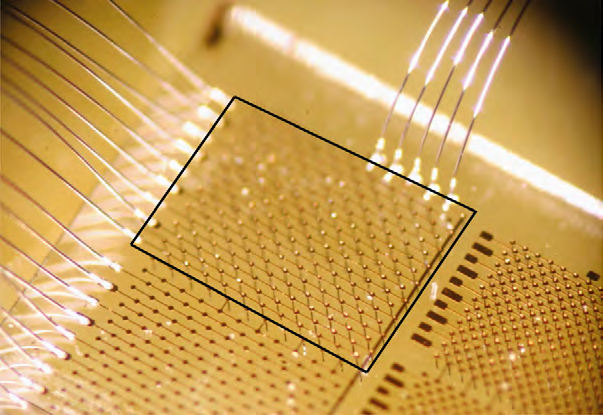
\includegraphics[height=0.4\textheight]{3D}
				\caption{prototype}
			\end{subfigure}
			\begin{subfigure}{0.45\textwidth} 
				\centering 
				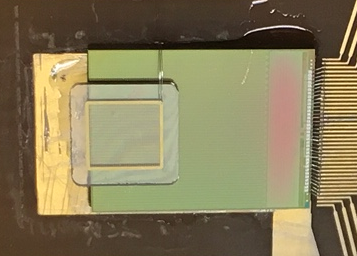
\includegraphics[height=0.4\textheight]{diapix}
				\caption{on CMS-Pixel chip} 	
			\end{subfigure} 
			\caption{3D diamond detectors} 
		\end{center}
	\end{figure}
\end{frame}
% ============== new frame
\subsection{Diamond as detector material}
\begin{frame}
	\frametitle{Diamond as detector material}
	\begin{itemize}
		\setlength{\itemsep}{\fill}
		\item \textcolor{cadmiumgreen}{$7-10$ times smaller charge loss due to radiation damage than in silicon}
		\item \textcolor{red}{signals (electrons created by a charged particle) half the size of silicon}
		\item $\rightarrow$ diamond becoming superior than silicon at a certain irradiation
		\item other advantageous properties:
		\begin{itemize}
			\item isolating material \ra negligible leakage current \ra power saving 
			\item high thermal conductivity \ra heat spreader for electronics
			\item large band gap \ra no cooling required
			\item high charge carrier mobility \ra fast signals
			\item working principle like a solid state ionisation chamber \ra no pn-junction required
		\end{itemize}
		\item disadvantages:
		\begin{itemize}
			\item high price
			\item some not fully understood behaviours 
		\end{itemize}
	\end{itemize}
\end{frame}
% ============== new frame
\subsection{Artificial diamond types}
\begin{frame}
	\frametitle{Artificial diamond types}
	\begin{itemize}
		\item used diamonds are artificially grown with a chemical vapor deposition (CVD) process
		\item investigation of two different diamond types:
	\end{itemize}
	\begin{figure}[htbp] 
		\begin{center}
			\begin{subfigure}{0.45\textwidth}  
				\centering 
				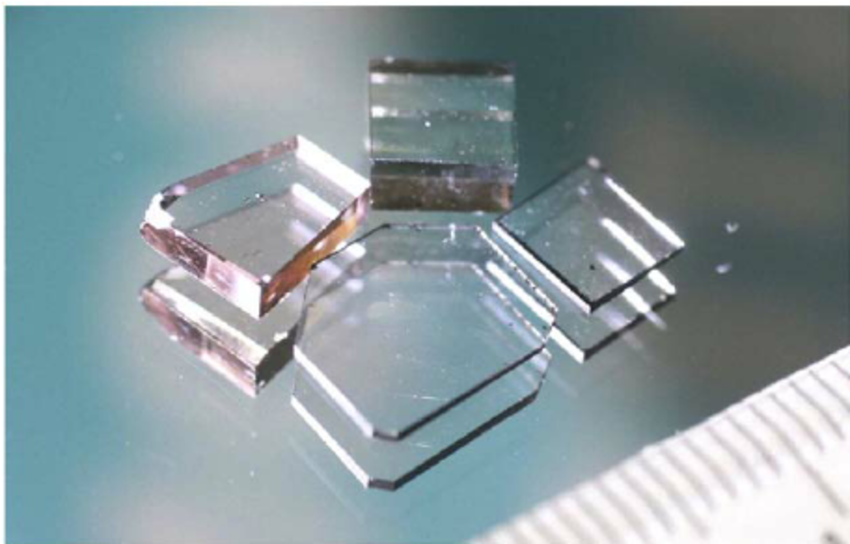
\includegraphics[height=0.4\textheight]{SCVD}
				\caption{single crystal CVD}
			\end{subfigure}
			\begin{subfigure}{0.45\textwidth} 
				\centering 
				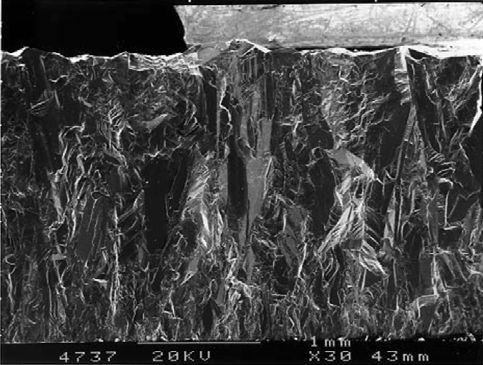
\includegraphics[height=0.4\textheight]{PCVD}
				\caption{poly crystal CVD} 	
			\end{subfigure} 
		\end{center}
	\end{figure}
	\begin{minipage}{5.5cm}
		\begin{itemize}
			\item grown on existing diamond crystal
			\item only small sizes (\SI{\sim.25}{cm^2})
			\item larger signals than pCVD ($5:3$)
		\end{itemize}
	\end{minipage}
	\hspace*{2pt}
	\begin{minipage}{5.5cm}
		\begin{itemize}
			\item grown on Si substrate with diamond powder
			\item large wafers (\SIrange{5}{6}{cm} \diameter)
			\item non-uniformities and grains
		\end{itemize}
	\end{minipage}
\end{frame}
% ============== new frame
\begin{frame}
	\frametitle{Diamonds in CMS}
	\begin{itemize}
		\item scCVD diamond pixel detector used in Pixel Luminosity Telescope (PLT)
		\begin{itemize}
			\vspace*{2pt}
			\item goal: stand-alone luminosity monitor for CMS
		\end{itemize}
		\item \textcolor{red}{observation of a signal dependence on incident particle rate:}
	\end{itemize}
	\begin{center}
		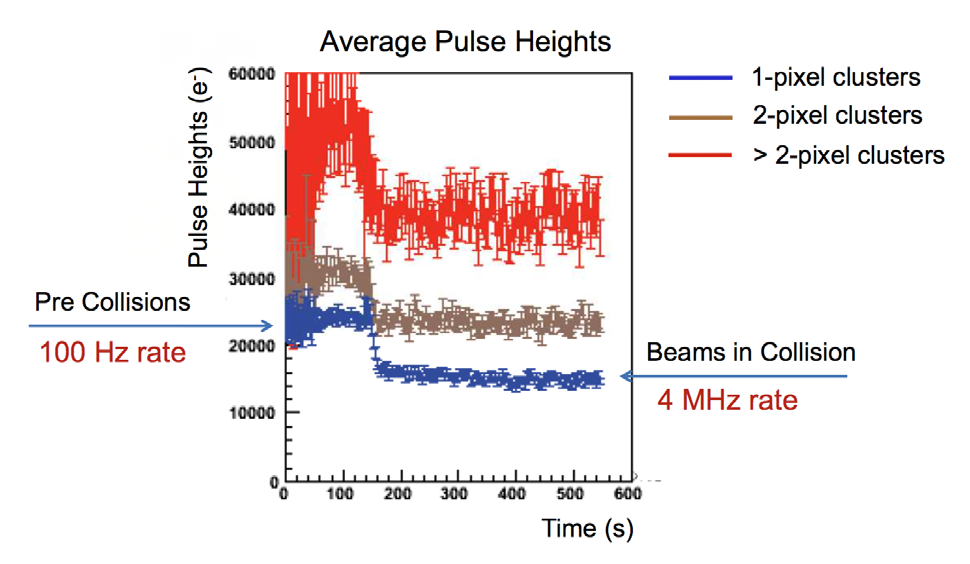
\includegraphics[width=7cm]{plt}
	\end{center}
	\vspace*{-15pt}
	\textbf{Consequences:}
	\begin{itemize}
		\item investigation of the rate effect in scCVD diamonds
		\item using pCVD diamond and prove that they show no rate dependence 
	\end{itemize}
\end{frame}

